\section{Sitting/standing position}

\begin{figure}[h]
  \begin{subfigure}[b]{0.45\textwidth}
    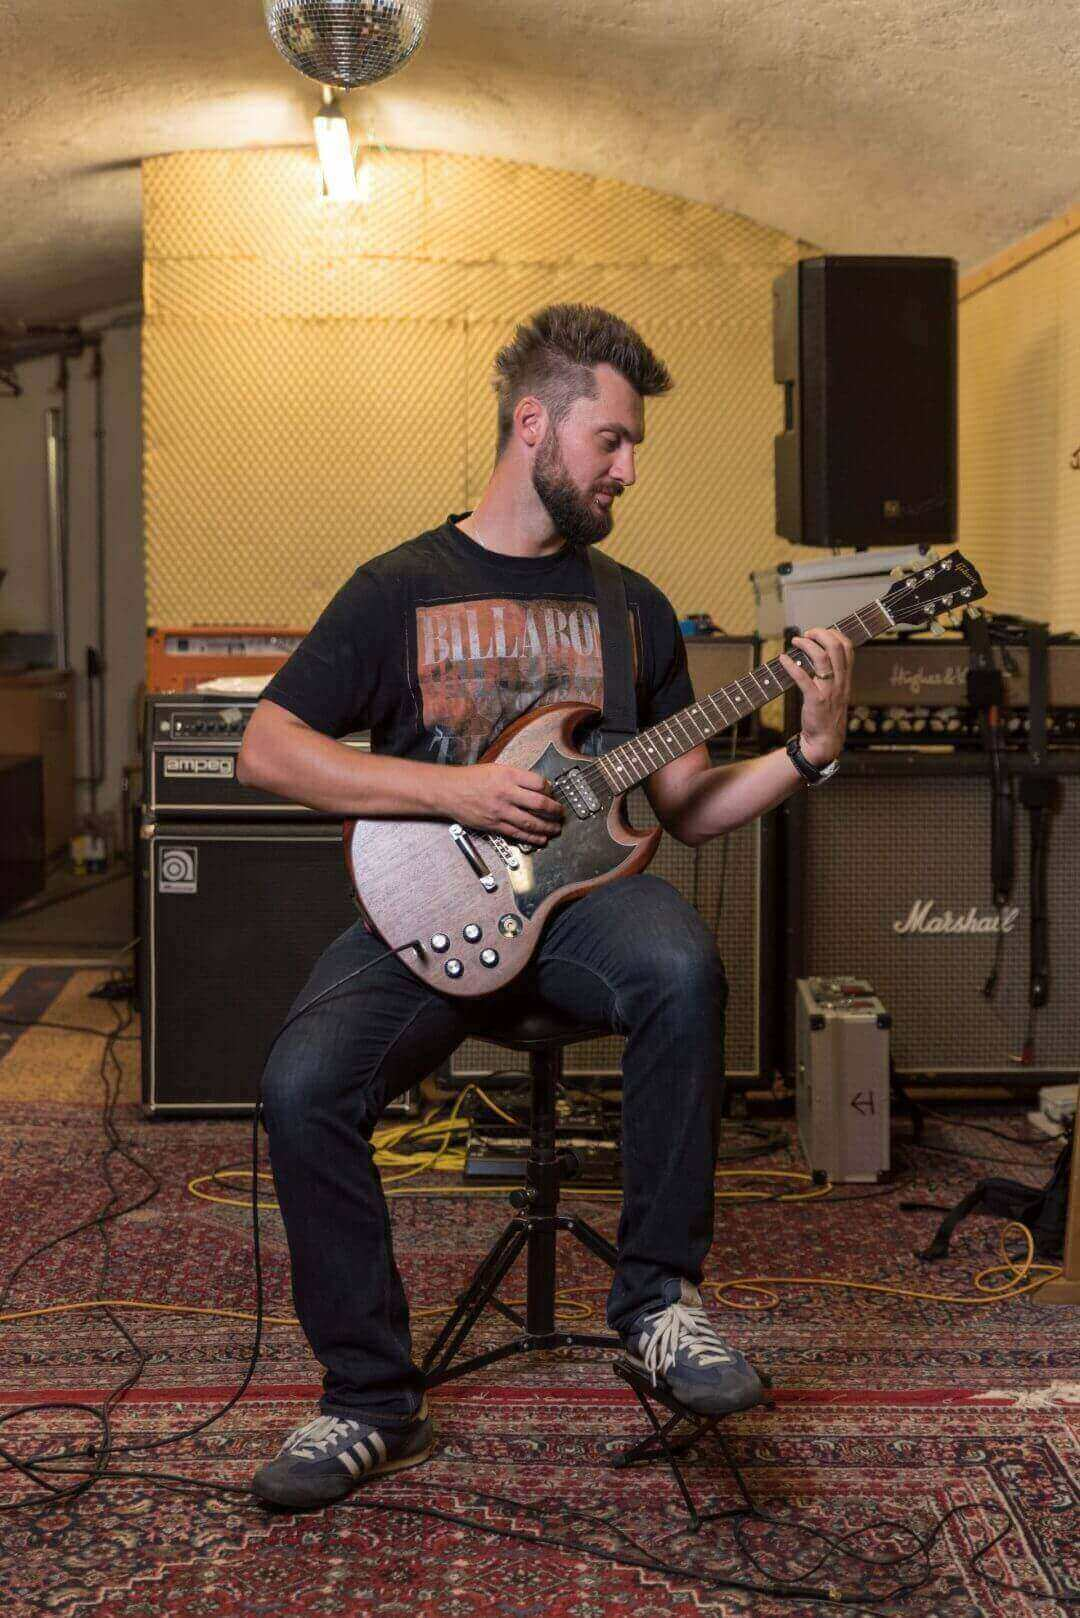
\includegraphics[width=\textwidth]{../Images/Letty_Guitar-Shooting_sitting.jpg}
    \caption{}
    \label{fig:positin_sitting}
  \end{subfigure}
  \hfill
  \begin{subfigure}[b]{0.45\textwidth}
    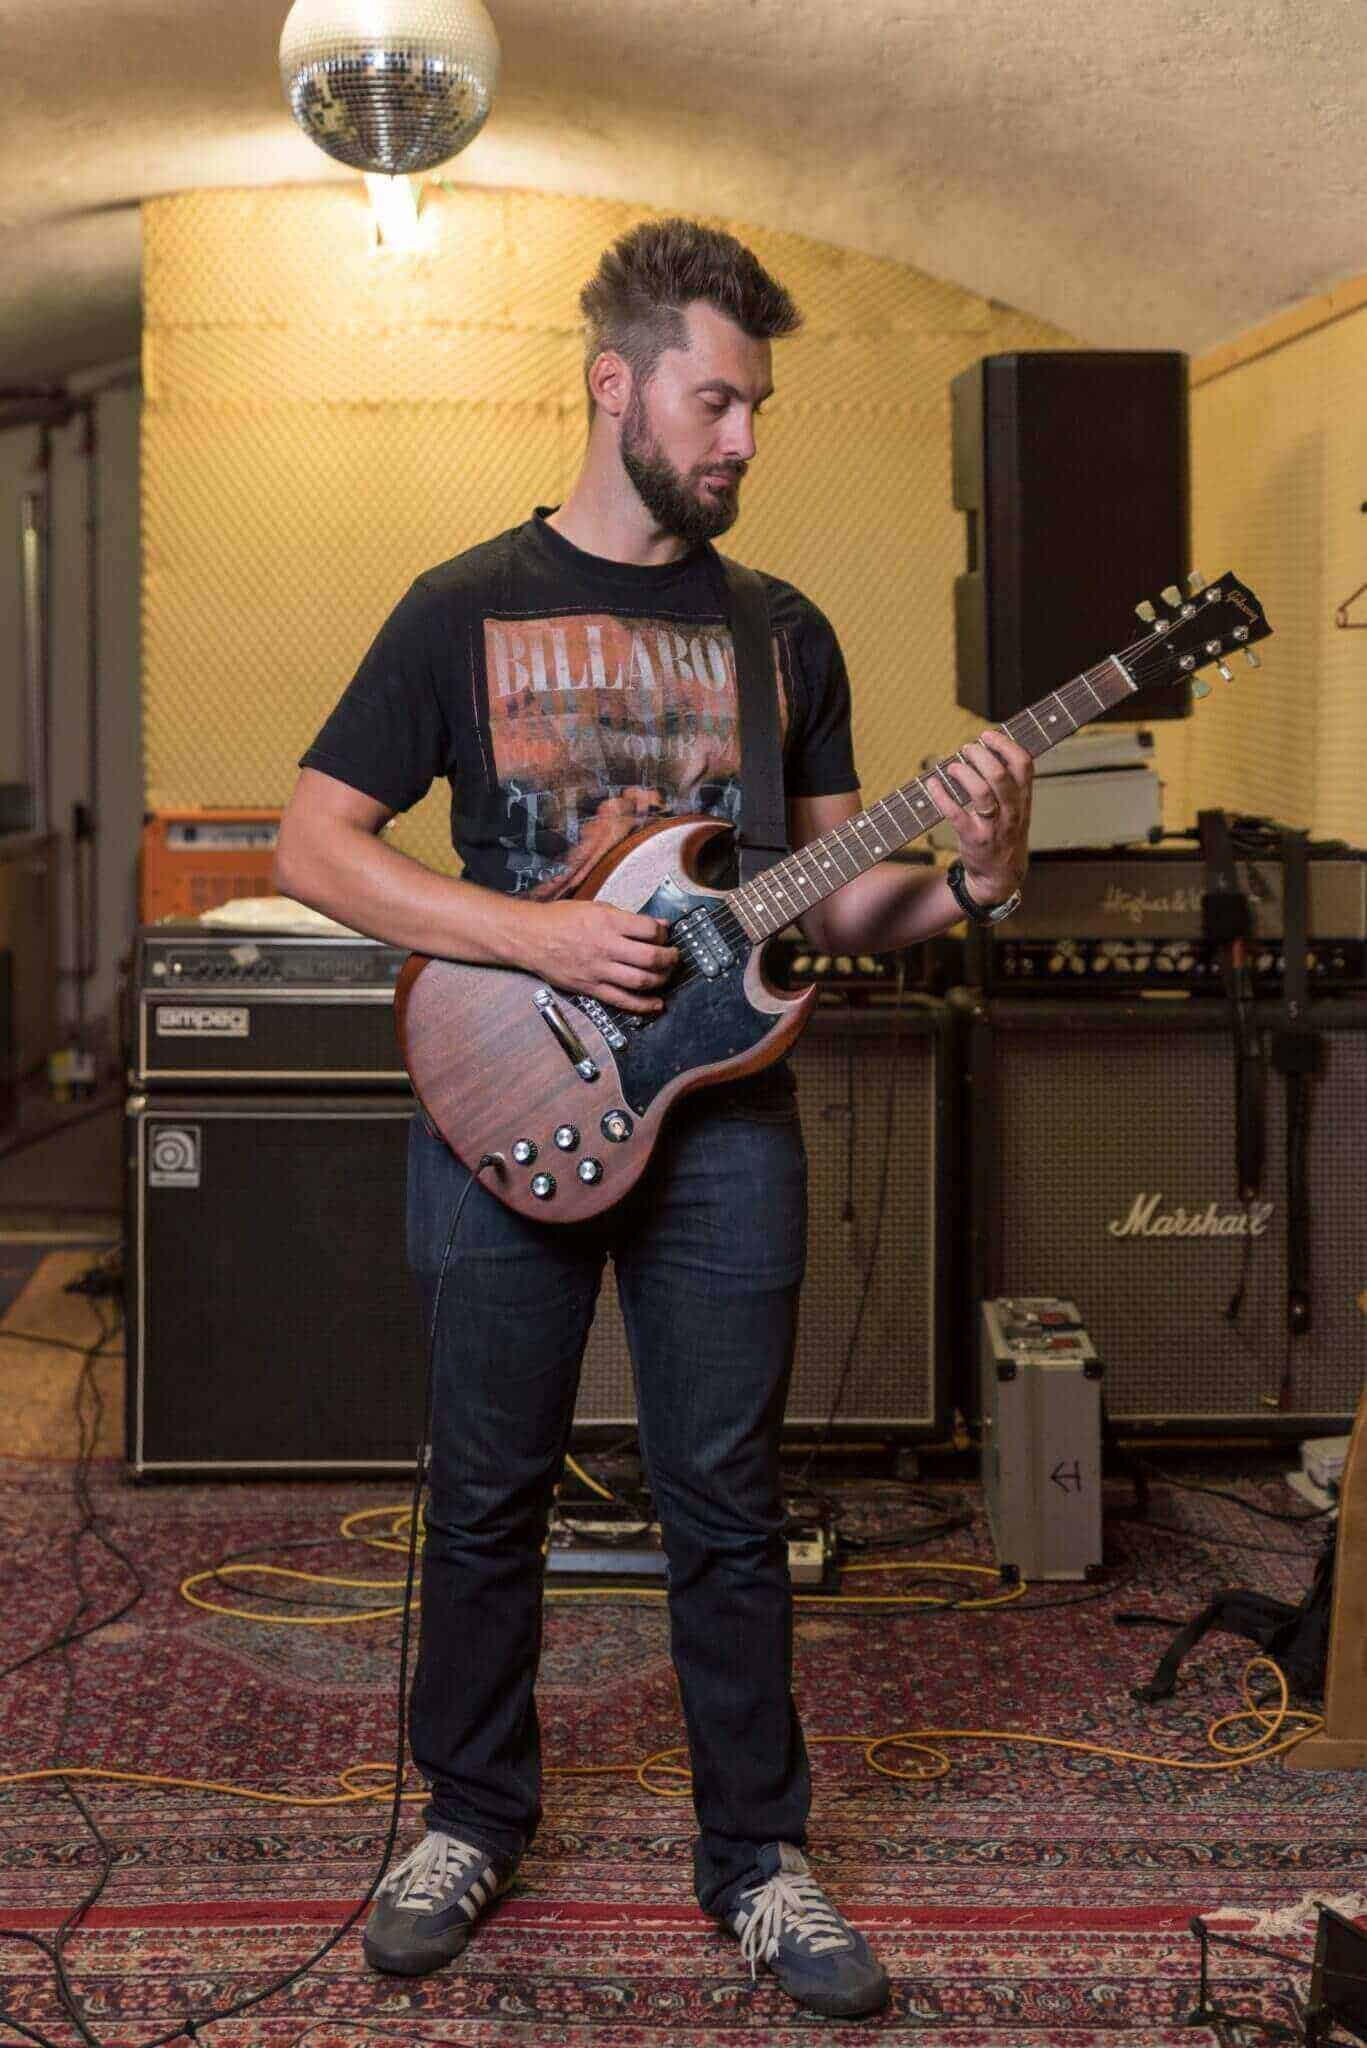
\includegraphics[width=\textwidth]{../Images/Letty_Guitar-Shooting_standing.jpg}
    \caption{}
    \label{fig:positin_standing}
  \end{subfigure}
  \caption{\cite{SitStandPosition}}
  \label{fig:positin}
\end{figure}

\infobox{This method assumes a right-handed player. If you are left-handed, replace “right” with “left” and vice versa.}

Even though it may look cooler to place the guitar on your right leg. You will be more comfortable and precise when you are sitting the classical way. The classical way of sitting also translates better to a standing position (see \ref{fig:positin_standing}).

In the classical position you place the guitar on your left leg and the left leg will be slightly raised. You can use a foot stool this this (see the leeft foot in \ref{fig:positin_sitting}).